\documentclass[onecolumn, draftclsnofoot,10pt, compsoc]{IEEEtran}


\setlength{\parindent}{0em}
\setlength{\parskip}{1em}
\usepackage[margin=0.75in]{geometry}
\geometry{textheight=9.5in, textwidth=7in}
\usepackage{listings}
\usepackage{imakeidx}
\usepackage{graphicx}
\usepackage{float}
\usepackage{listings}
\usepackage{hyperref}
\usepackage{url}
\usepackage{longtable}
\usepackage{enumitem}
\usepackage{setspace}
\singlespacing



\def \DocType{	
	
	FINAL REPORT	
}


\lstset{
  basicstyle=\small\ttfamily,
 numbers=left,
  numberstyle=\scriptsize,
  showspaces=false,
  showstringspaces=false,
  breaklines=true
}





% 1. Fill in these details
\def \CapstoneTeamName{DSCVL-Overcomers}
\def \CapstoneTeamNumber{69}
\def \GroupMemberTwo{LUCIEN-ARMAND T. TAMNO}
%\def \GroupMemberThree{			}
\def \CapstoneProjectName{Depth sensing with computer vision and lidar}
\def \CapstoneSponsorCompany{}
\def \CapstoneSponsorPerson{ D. Kevin McGrath}


\usepackage{datetime}
\newdate{date}{12}{6}{2018}
\date{\displaydate{date}}

\title{\centering
			
\includegraphics[height=4cm,natwidth=200,natheight=300]{images/osu_logo.eps}\\\vspace{.5in}
		\scshape{\huge CS CAPSTONE \DocType \\\vspace{.5in}
		\textbf{\Huge\CapstoneProjectName}\\\vspace{1in}
		\large	\displaydate{date}\\\vspace{.3in}		
			\large {Prepared For}\\\vspace{.1in}
			\textbf{{\Large \CapstoneSponsorPerson}} \\\vspace{.6in}		
				\large {By} \\\vspace{.1in}
				\textbf {Group \CapstoneTeamNumber}\\\vspace{.1in}
				\large {\CapstoneTeamName}\\\vspace{.1in}
				\textbf{ { \GroupMemberTwo}}
}  
}

\IEEEtitleabstractindextext{
 \begin{abstract}
This Depth Sensing with Computer Vision and Lidar report describes  the project development from its historical genesis to the final result. The report includes the chronological development,shareholders, participants and their different roles,  technical and management skills learned, as well as reflections.  
 \end{abstract} 
 
}
%%%%%%%%%%%%%%%%%%%%%%%%%%%%%%%%%%%%%%%

\begin{document}
\pagenumbering{gobble}
\maketitle
\IEEEdisplaynontitleabstractindextext
\IEEEpeerreviewmaketitle
\newpage
\pagenumbering{arabic}
\tableofcontents
\newpage
	
\section{Table of Contents}
\tableofcontents
\bibliographystyle{IEEEtran}
\bibliography{ref}


 
\begin{singlespace}
	\section{Definitions}
			\textbf{IR: }\label{def:IR}\par
		IR stands for the infrared technology.

		\textbf{IR Depth Sensor: }\label{def:depthsensor}\par
		A device that calculates distances by emitting infrared signals. 
		
		\textbf{LIDAR: }\label{def:lidar}\par
		Light Detection And Ranging - A method that uses lasers to measure distance
		
		\textbf{Microsoft Kinect: }\label{def:kinect}\par
		A product that uses an IR Depth sensor to measure distances.
		
		\textbf{Logitech Brio Webcam: }\label{def:brio}\cite{logitech}\par
		The webcam model this project shall be using.
		
		\textbf{RPLidar A1: }\label{def:rplidar}[1]\cite{slamtec}\par
		A low-cost LIDAR unit that this project shall be using.
		
		\textbf{RPLidar Solid-state: }\label{def:rplidar2}\cite{leddartech}\par
		A High-cost LIDAR unit single direction with better performances of detecting, measuring and locating liquids and people
	 	
		
		\textbf{Computer Vision: }\label{def:vision}\par
		The methods for acquiring, processing, analyzing, and classifying digital images and extracting information.
		
		
		
		\textbf{Python/C API: }\label{def:API}\cite{Ctype}\par
		API: application programming interface between Python and C programs
		
		\textbf{DSCVL: }\label{def:DSCVL}\par
		Acronym that stands for Depth sensing with computer vision and lidar

\end{singlespace}

		
		
	\section{Introduction}
	The DSCVL project today a solution, was originally our client idea to have  a new technology by overlaying two signals from different sources. The first signal  being captured the existing Lidar technology and the second signal coming from a camera technology. Therefore, the goal of project was to turn the descriptive above concept in a viable application to address the gap left by the infrared technology in outdoor environment.
	
 In fact, the Lidar technology is  reliable in outdoor environment and capable to provide with precision objects distance measurements. And one of the reliable device uses by this technology is the  16-Segment SOLID-STATE Lidar equipment, at times called the Leddar M16 \ref{def:rplidar2}. The second technology we use in this project is the  webcam  specifically the Logitech Brio Webcam \ref{def:brio} and it is used to get images.  
  
More importantly, the fact that the lidar technology ( Leddar M16) was more reliable to provide better objects measurements than the IR technology \ref{def:IR}, was presented to us the ideal technology of choice. so both, Lam and I as suggested by Kevin our client, decided to use it.

\section{Current State of the DSCVL}
Though, the past winter term progress report described the RPLidar A1 capability  \ref{def:rplidar} of outputting  useful information but the reality is that the DSCVL project  needed some changes for the sake of better accuracy. some changes took place at different level of the project. And the most important being the replacemnt of RPLiadr A1 by the 16 segment solid state M16 that provides better detection, localization, and distance measurements when is to compares to the RPLidar A1.\par

Additionally, those differences can even be more tangible at the code level, because the M16 model has its code literally written in C program while the RPLidar code is closely related to the python environment. And this M16 factor code-based caused me to conduct researches to figure out how can I make the C program code work in python environment. The result of that research was to discover the python \ref{Ctypes} functionality to play the intermediary role of having the C program code runs in a python environment.With the same idea, I dug a little bit more to finally find out that Visual Studio is the suitable Windows application to implement the python/C API.  

 
\subsection{ Preliminaries and the Python/C API implementation}
	\subsubsection{Are there any special hardware, OS, or runtime requirements to run your software?}
To run the  Leddar M16 technology, I have to implement the python/c API\ref{def:API} using the C-code that was shipped with the M16 device. And to do so, I have to make sure first that  the M16 can properly run in a Windows environment by default. And for me to test that functionality, I installed and configured the default M16 settings, as shown in figure \ref{signal} below.

   \begin{figure}[H]
			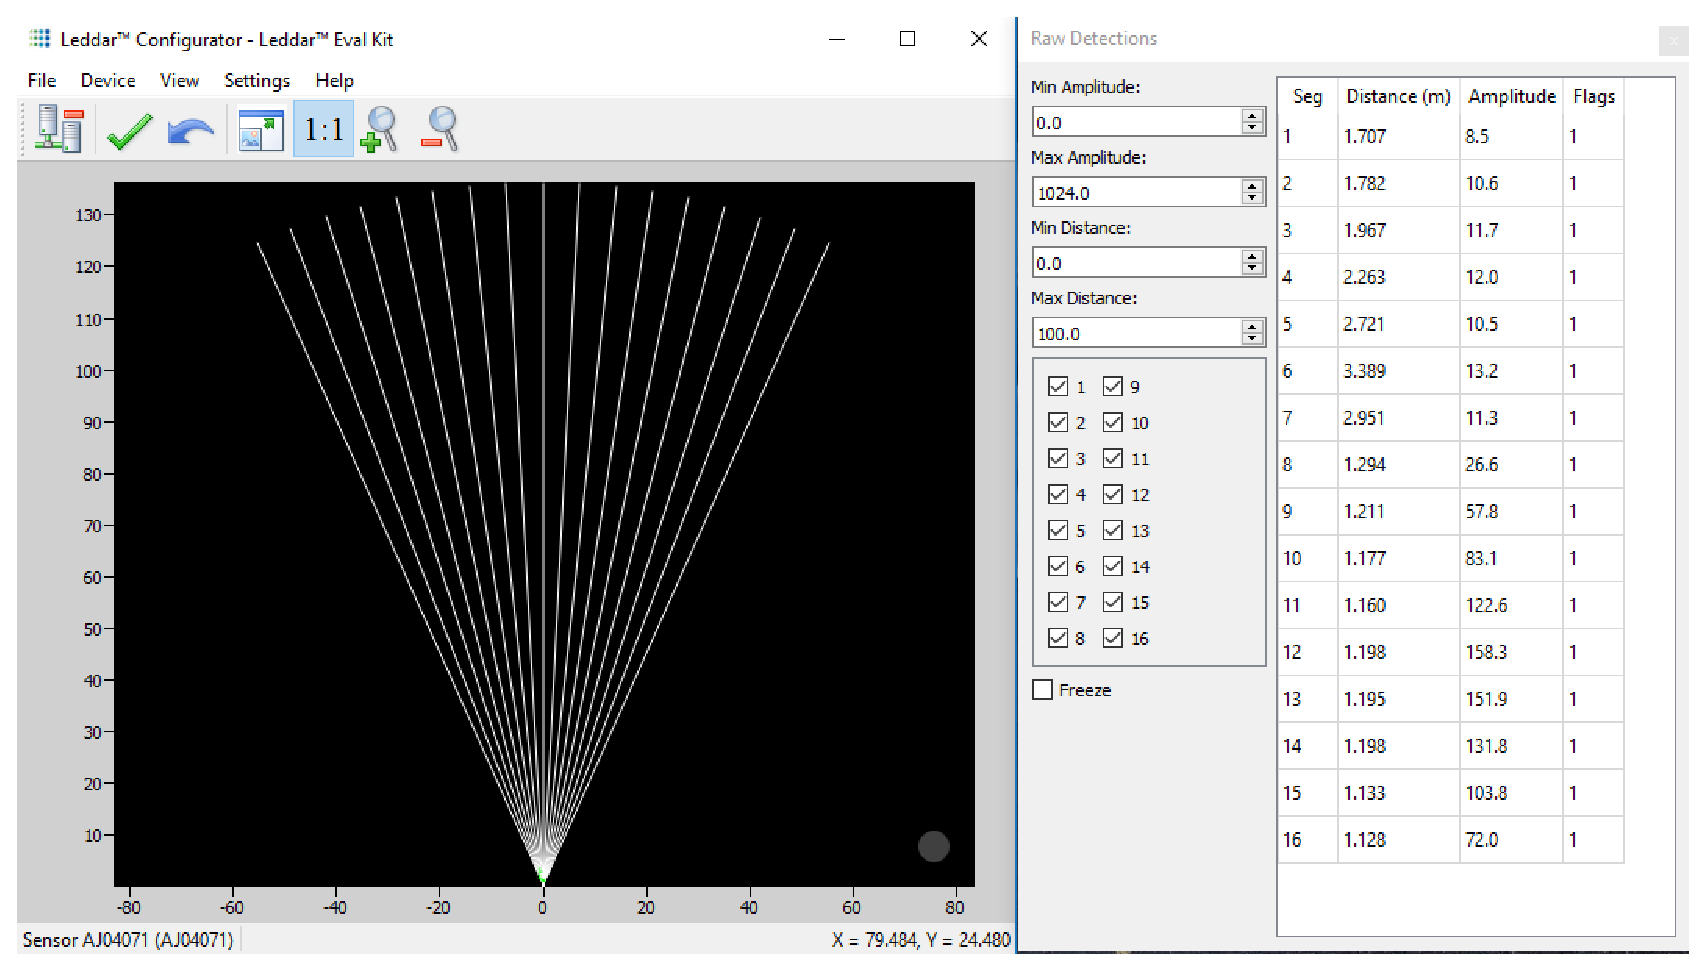
\includegraphics[scale=0.5]{images/signal.eps}
			\caption{figure}{Leddar M16 outputs distance measurements  using the default windows installation [right] and default M16 screen [left].}
			\label{signal}
		\end{figure}
		
That figure \ref{signal} displays a sample distance outputs as it is supposed to be visualized by a user at the final stage of the DSCVL project. Though, differences may be seen in term of data disposition on the screen,because the M16 code has to run in conjunction with webcam technology to overlay images form the python environment. Hence, the implementation of the DSCVL application has an additional technological constraint to be done via an API.
		
		\subsubsection{How does your project work?}
		
To get the written C++ language code to python, the Visual studio 2017 application was the relevant tool to use. Therefore, I installated  visual Studio in Windows 10 system, imported any necessary library to connect the visual Studio  to the Leddar M16 C-code,using the appropriate \cite{Microsoft} documentation related to the topic. 
The remaining bulk of work is  to write and debug the API implementation code to make sure the M16 interacts properly from the visual studio perspective and secondly, to integrate in a single package the python and the M16 C codes, as shown in figure \ref{python-Cpp}.

 \begin{figure}[H]
			\includegraphics[scale=0.5]{images/python-Cpp.eps}
			\caption{figure}{Python/C API built in Visual Studio 2017.}
			\label{python-Cpp}
		\end{figure}
		
		
However, when working on the  above API, I encountered multiple setbacks.among others, the two most important issues are:the slight Leddar M16  differences seen in the the M16 files, for instance I had to change one default header, as shown in figure \ref{change-M16} below.

 \begin{figure}[H]
 \centering
			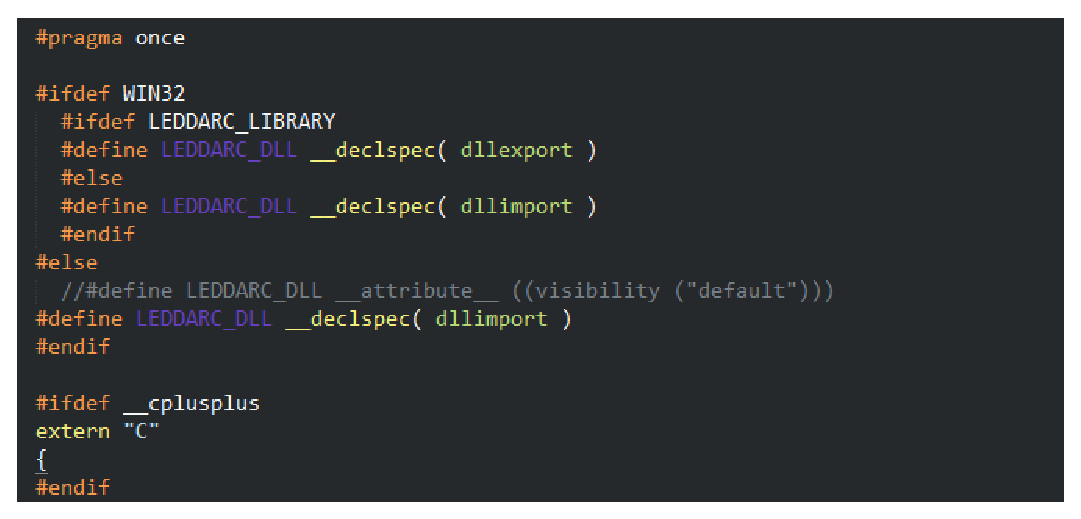
\includegraphics[scale=0.5]{images/change-M16.eps}
			\caption{figure}{Snippet code changed in the Leddar M16 header file.}
			\label{change-M16}
		\end{figure}

And the worst being found in the current debugging phase that presents a successful result in code checker but generates several linkage errors.  

Finally, I also wrote an additional decorator function in the python module to speed up the python execution module as shown in figure \ref{change-M16}here underneath.

 \begin{figure}[H]
 \centering
			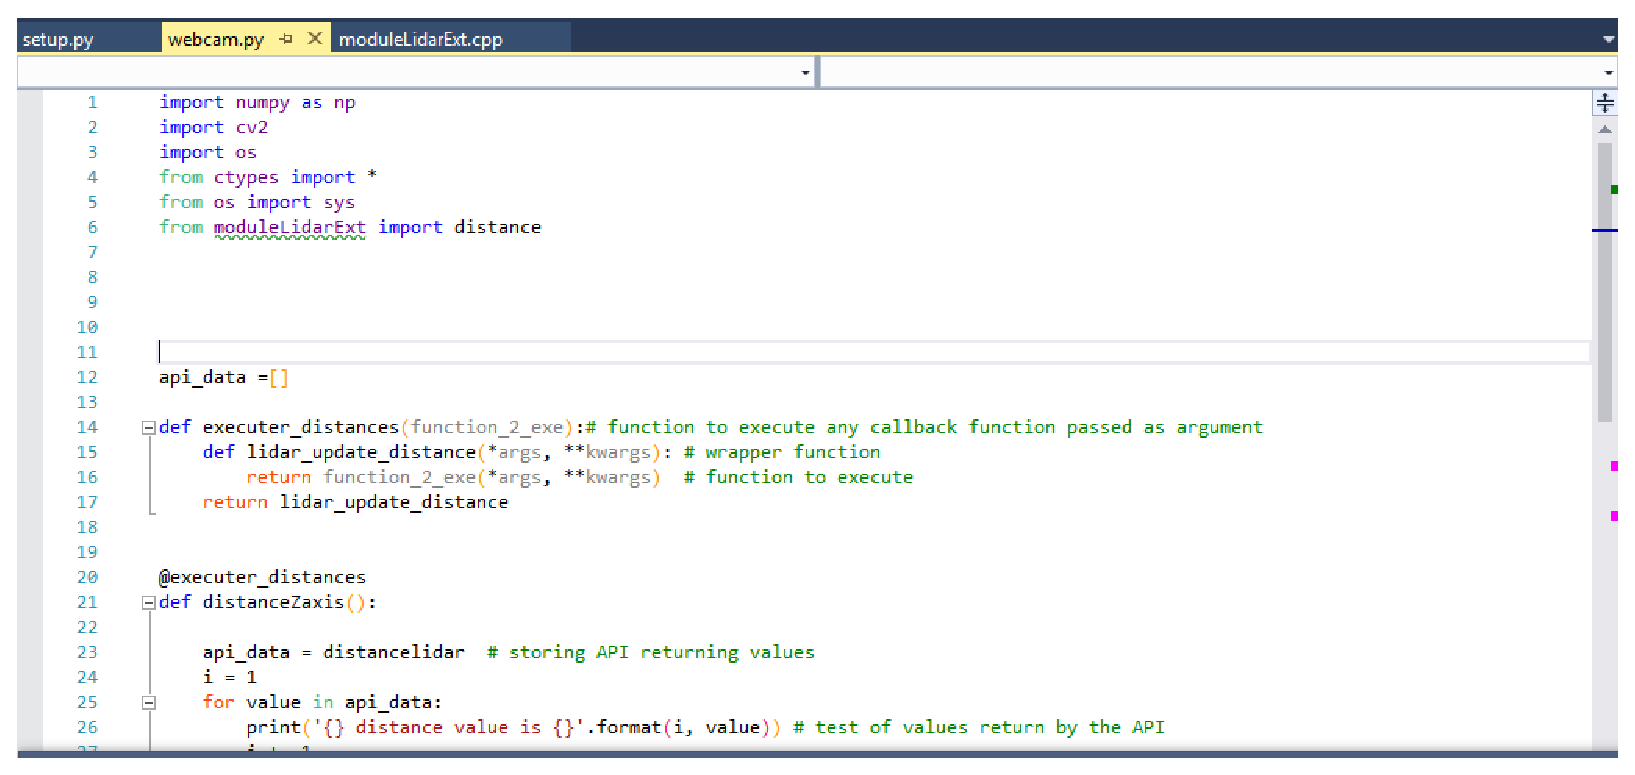
\includegraphics[scale=0.5]{images/python-ext.eps}
			\caption{figure}{Python decorators code.}
			\label{python-code}
		\end{figure}
		
		
\subsection{ Legacy: GUI Interface}

In order to prioritize the DSCVL backend, the Frontend was relegated because the backend is more important and represent the project core functionality as envisioned in the final stage. The GUI downgrade, yet still provides the basic services it has before, but it is not clear whether the final DSCVL system would make use of the legacy graphical user interface.
		
		 

\section{Final Gantt Chart}

 \begin{figure}[H]
 \centering
			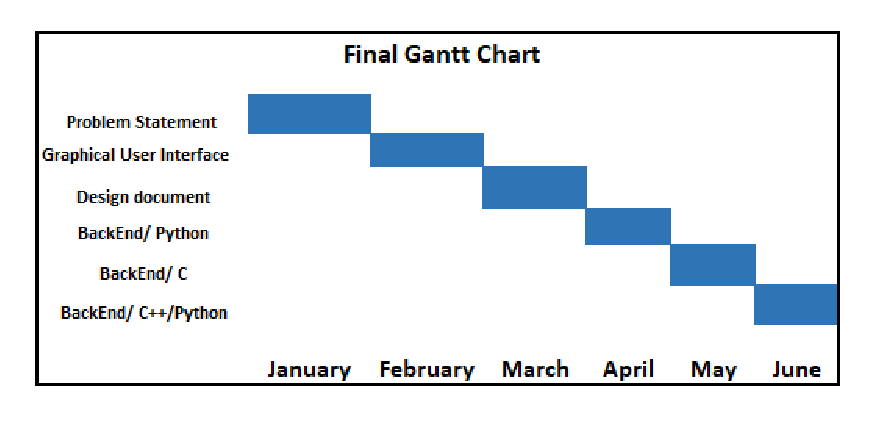
\includegraphics[scale=1]{images/gantt.eps}
			\caption{figure}{Final Gantt Chart}
			\label{gantt}
		\end{figure}
			
\section{Design Document}

\include{designdocument}

\section{Weekly Blog Posts over six Months}
	\subsection{Ten-Week Term Retrospective}
		\begin{longtable}{|l|p{0.3\linewidth}|p{0.3\linewidth}|p{0.3\linewidth}|}\hline \textbf{Week} & \textbf{Positives} & \textbf{Deltas} & \textbf{Actions}\\\hline
		1-Jan 	& - & - & -\\\hline

		2-Jan 	&
\begin{itemize}
\item back and forth email communication with Kevin regarding to way to get into the CS 462 and CS 406 
\end{itemize}
			&
\begin{itemize}
\item Kevin emailed me back regarding the way i wanted to work in a new project: to whether i have decided to work with a partner or to do it in solo.
\item The next day exactly on Friday, January the 19th he informed me that he is making an arrangement.
\end{itemize}
			&
\begin{itemize}
\item I emailed Kevin to know what would the next step after registering to the cs 406 and cs 462.
\item I replied to Kevin that " working with a partner would be beneficial to me and allow to simulate   a real-world experience.
\end{itemize}

			\\\hline

		3-Jan	&
\begin{itemize}
\item This week, the Group 69 is born
\item For the first time I had a fruitful exchange with my partner Lam
 
\end{itemize}
			&
\begin{itemize}
\item At this point, I did not know to jump onboard and get started with the project though i could note a positive interaction with Lam.
\end{itemize}
			&
\begin{itemize}
\item i reached Lam out to get the insight about the new project and for the first amazingly, the promptly respond to my email by outlining the key points of the Depht sensing with computer vision and lidar project, which at that times was titled ROS lidar project.
\item I was encouraged by Lam to reach out Junki as he was introduced to us by Kevin as our  TA and ultimately Junki accepted to be our TA.
 
\end{itemize}
			\\\hline

		4-Jan	&
\begin{itemize}
\item if week 3 was the week that our group was born, week 4 actually indicates when i effectively got started on searching what could be one way of solving the DSCVL problem.
\end{itemize}
			&
\begin{itemize}
\item I got into my first struggle trying to install the python libray on Windows 10
\item I had no idea how to get the rplidar library worked on Windows.  

\end{itemize}
			&
	\textbf{ weekly tasks list}  	
\begin{enumerate}
\item Install RPLiar python library [5]
\item Build the appJar  file from the appJar library for the GUI [3] 
\end{enumerate}
			\\\hline

		5-Fev 	&
\begin{itemize}
\item noticeable progress done by building python libraries and configuring paths to properly work in windows environment 
\end{itemize}
			&
\begin{itemize}
\item I met with Kevin during the weekly office hour session and put forward an sketched figure of how I was designing  final overlay image and also how would the relative distance of the object to be captured by the Robotpeak lidar device. 
\end{itemize}
			&
	\textbf{ weekly tasks list}
	\begin{enumerate}
	\item Download and install Numpy  wheel files
	\item Download and install OpenCV wheel file
	\item Configure " pip" tool to run with the Windows 10
	\item explore how to work with tkinter library  
	\end{enumerate}

			\\\hline

		6-Fev	&
\begin{itemize}
\item week for the midterm progress report write up
\item built the pdf slide presentation file along with its video
\end{itemize}
			&
\begin{itemize}
\item 
\end{itemize}
			&
			\textbf{ weekly tasks list}
\begin{enumerate}
\item 	Turn in midterm process report ( slide, write up, audio recording)
\item wrote the first function to capture the video stream from the my built-in webcam and store images on the Hard drive.
\end{enumerate}
			\\\hline

		7-Fev	&
\begin{itemize}
\item explore other possibilities to build a virtual Linux layer on top of the windows OS.
\item work with the Group 40 learder to have a private critique poster session
\end{itemize}
			&
\begin{itemize}
\item Faced a serious setbadk to make the windows 10 system work with the rplidar device. 
\item I was having buggy results regardless changes made in the source code program
\end{itemize}
			&
			\textbf{ weekly tasks list}
\begin{enumerate}

\item Read documentation to perform test reading from the lidar device
\item Helped out by Kevin to successfully read data from the  lidar A1 scanner
\end{enumerate}

			\\\hline

		8-Fev	&
\begin{itemize}
\item we missed the class poster critique session, and planned to attend the one with Group 40.
\end{itemize}
			&
\begin{itemize}
\item 
\end{itemize}
			&
			\textbf{ weekly tasks list}
\begin{enumerate}
\item raised questions that prompted me to go back and take a closer look at how the rplidar A1  is trying to read data and how i can utilize those data for Z-axis calculations.
\end{enumerate}
			
			\\\hline

		9-March	&
		\begin{itemize}
		\item Poster Critique session meeting in Kelly Hall with Kirsten as supervisor,  Group 40 team.
		\item outcomes of the session/ poster format correction: the need of labeling the central image with axis was presented, Include group members contact  information if necessary and include the client of the project.
		\item explored some the benefits of the Tensorflow technology and in particular the "eager execution" version   
		\end{itemize}

			&
\begin{itemize}
\item  I Was told by Junki and Lam that Tensorflow will not be helpful for the z-axis calculus.
\end{itemize}
			&
			
			\textbf{ weekly tasks list}
\begin{enumerate}
\item contact Nathan leader of Group 40 for the final arrangement for the critique session
\item loop back to update my team partner Lam abot the critique session.
\item i successfully wrote functions to turn rplidar stream data into an array of float values. And then, for that array of float points to be array of values to represent the mobility of the object in front of the lidar device.
\item Install of the eager execution python wheel file on windows 10 
\end{enumerate}
			\\\hline

		10-March	&
\begin{itemize}
\item compute the z-axis object movements using geometrical maths functions
\item explore how i would be using the numpy spacial functions to get around with the standard maths functions [6]
\end{itemize}
			&
\begin{itemize}
\item Still struggling to transform the array float points of data into 2-D array to pass it as one of arguments for the  numpy function.  
\end{itemize}			
			
			&
			\textbf{ weekly tasks list}
	\begin{enumerate}
	\item  Install spicy spacial numpy wheel file on windows 10
	\item write the final winter progress report 
	\item write the slide of the report presentation and build the video
	\
	\end{enumerate}

			\\\hline
			
					11-Apr	&
\begin{itemize}
\item read  the python documentation for C extension
\item explore the possibility to use command line for module extension
\end{itemize}
			&
\begin{itemize}
\item still unable to clearly understand how   C can be extended in python.  
\end{itemize}			
			
			&
			\textbf{ weekly tasks list}
	\begin{enumerate}
	\item  search more info in the python documentation
	\item  find information about static libray 
	\end{enumerate}

			\\\hline
			
					12-Apr	&
\begin{itemize}
\item Find out website to provide samples of project where dynamic Library C/python is used in command lines.
\end{itemize}
			&
\begin{itemize}
\item Still do not know how to interpret  data form the M16 documentation.  
\end{itemize}			
			
			&
			\textbf{ weekly tasks list}
	\begin{enumerate}
	\item  Download and Install of the Leddar M16 exe file for Windows 10 (64 bits)
	\item Configuration of the M16 in Windows 10 environment 
	\item Import the Ctypes function library in python  
	\
	\end{enumerate}

			\\\hline
			
					13-Apr	&
\begin{itemize}
\item commands to Create a dynamic library to link files in Linux
\item  commands how to compile dynamic library in Linux 
\end{itemize}
			&
\begin{itemize}
\item    keep searching how to implement DLL in Windows  
\end{itemize}			
			
			&
			\textbf{ weekly tasks list}
	\begin{enumerate}
	\item  save all the linux commands for DLL
	\item  sample command:  and gcc -shared -o  lnkfile.so file1.c file2.c  ..filex.c
	\end{enumerate}

			\\\hline
			
					14-Apr	&
\begin{itemize}
\item Get the main website describing how to create C extension in python
 
\end{itemize}
			&
\begin{itemize}
\item confront to the problem of Visual Studio.  
\end{itemize}			
			
			&
			\textbf{ weekly tasks list}
	\begin{enumerate}
	\item  Install Visual Studio But computer freezes 
	\item Perform some extra work on the computer to keep on with the project
	
	\end{enumerate}

			\\\hline
			
					15-May	&
\begin{itemize}
\item 
\item Explore other possibilties to call Leddar M16 function.
\end{itemize}
			&
\begin{itemize}
\item  Erreur prompt by visual studio on the C function called
\end{itemize}			
			
			&
			\textbf{ weekly tasks list}
	\begin{enumerate}
	\item  determine what function C to run on API  
	\item Define of the module python on visual studio 2017  
	\item document the first process to call function in Visual Studio
	\
	\end{enumerate}

			\\\hline
			
					16-May	&
\begin{itemize}
\item  examine how to include and link SDK files in Visual Studio (VS)
\end{itemize}
			&
\begin{itemize}
\item  Still facing failure issue at the python/C API and VS  
\end{itemize}			
			
			&
			\textbf{ weekly tasks list}
	\begin{enumerate}
	\item  Headers importation in VS
	\item  Write some main function in the API module
	 
	\end{enumerate}

			\\\hline
			
					17-May	&
\begin{itemize}
\item  explore other paths of writing the API 
\end{itemize}
			&
\begin{itemize}
\item drawback, the Seasnake  implemenmtation could not work in VS 2017
\end{itemize}			
			
			&
			\textbf{ weekly tasks list}
	\begin{enumerate}
	\item Get around the Visual Studio issues of  linkage
	\item Attempt to use seasnake 
	\item document seasnake installation process
	\item Keep working on the previous Python/C API
	\end{enumerate}

			\\\hline
			
					18-May	&
\begin{itemize}
\item  Explore every single possibility to include SDK in VS   
\end{itemize}
			&
\begin{itemize}
\item Struggle with Windows System errors and problems of machine failure.   
\end{itemize}			
			
			&
			\textbf{ weekly tasks list}
	\begin{enumerate}
	\item  Maintain Machine and re-install the environment Visual Studio Windows
	\item reconfigure the entire project
	\item  continue testing integration of the C Leddar in VS
	\item successfully include SDK links in linker
	\end{enumerate}

			\\\hline
			
					19-June	&
\begin{itemize}
\item successfully compile of the ptython/C++ API 
 
\end{itemize}
			&
\begin{itemize}
\item Struggle to call the function Leddar in python code  
\end{itemize}			
			
			&
			\textbf{ weekly tasks list}
	\begin{enumerate}
	\item  Include all headers in the C/API 
	\item Include all files in different modules  
	\item Include links and other files in the VS properties option
	\
	\end{enumerate}

			\\\hline
			
					20-June	&
\begin{itemize}
\item  Narrow the problem of the module python not validating extension at the visual studio level
 
\end{itemize}
			&
\begin{itemize}
\item   Module python still not working  
\end{itemize}			
			
			&
			\textbf{ weekly tasks list}
	\begin{enumerate}
	\item Write final report Presentation 
	\item write final winter progress report 
	\end{enumerate}

			\\\hline
			
		\end{longtable}


\subsection{How does one run it?}
The Python/C++ API run but the module python to handle the call function from API accuses a Windows Visual Studio issue.
 
\subsection{What web sites were helpful?}
This needs to be detailed enough to recreate and/or use your project!\par
\subsection{Recommended Technical Resources for Learning More}
To dive into this topic, one can use links provided in the appendix section to learn more about the topic.

\subsection{What web sites were helpful?}
The bulk of the this project from start to finish was mostly done using websites as listed underneath. the first set of websites consists of sites used to develop the Python/C API and the second set lists sites related to libraries for python module.
\subsubsection{websites for the python/Cpp API}
\begin{enumerate}
\item python/C++ API guidelines Using Visual Studio[1]
\item Download File Leddard M16 [2]
\item Install Visual Studio 2017 [3]
\item Building C and C++ Extensions[4]
\item  Foreign function  library for Python[5]
\end{enumerate}
\subsubsection{other libraries for python}
\begin{enumerate}
\item OpenCV[6]
\item Numpy [7]
\end{enumerate}



\subsection{reference books really Helped}
Basically,some of the books I was able to glimpse a book Advance C++ programming[8]. But as I have said it in the section website that helped the most and my research was carried out via internet, on Windows web pages, python repositories and others like Github repository.
 

\subsection{Other Party Involvement}
When is to say who else was involved in this project except my teammate, I have to admit the fact that our client was helpful by providing some guidelines and paths for me to look into. I received from our client the main website in which all the first instructions related to the python/C API implementation could be found. And from that point on, though most of the student did not have any past experience with python and C working in visual studio IDE, I found one graduate student o whom I showed the python error to recognize the extension module from C and He tried to provide some instructions unfortunately that did not work.


\section{Conclusion}
Over the course of this project I was able to the first able to implement resident application API in windows environment, integrate  python module in visual studio by specially customizing Python environment to work in Windows. Additionally, I was able to  to engage in research activities whenever the project was not working to get the project going by googling or reading in other material suitable for the area of the project.

For non-technical skills, I learned to work in a team by considering the perspectives of the other group member. But beyond that, I learned to ask help by clearly explaining to the person to whom I needed help from, the challenge I was facing. Due to the hidden hurdles that he project work presented to me. And to elaborate about the project work, one of the key point i would always remember is that a project does not only need technical skills to be successful, but also non-technical skills  as well. It is submitted to my attention to be solve  but more importantly, it is an opportunity to learn new skills, to explore new ways to work with others, to accept inputs from them changes and adapt to those transformations that presented to me either as an advice or a reproach. The latter, can only be possible in a teamwork environment and good management is the way to go. By Management I mean, to learn how to handle stress that can be imposed to you by the amount work to do or the speed at which that work has to be done.  

Finally, if I could go back and do this project all over this project, the first thing i would do is to get started on the python/C API because this module appear to be straightforward to implement but unfortunately that is not the case, Because the module has hidden aspects like how Visual studio interacts with Windows platform to provide services in python environment, which is one important phase of the python/C API development in Windows system. 


\section{Appendix}
[1]\hyperlink{https://docs.microsoft.com/en-us/visualstudio/python/working-with-c-cpp-python-in-visual-studio}{python/C++ API guidelines Using Visual Studio}

[2]\hyperlink{https://support.leddartech.com/downloads/files/91-leddarinstaller-exe}{Download File Leddard M16}

[3]\hyperlink{ https://docs.microsoft.com/en-us/visualstudio/install/install-visual-studio}{Install Visual Studio 2017}

[4]\hyperlink{https://docs.python.org/3/library/ctypes.html\# loading-shared-libraries}{Foreign function  library for Python}

[5]\hyperlink{https://docs.python.org/3/extending/building.html}{Foreign function  library for Python}

[6]: \hyperlink{https://www.lfd.uci.edu/\~gohlke/pythonlibs/\#opencv}{OpenCV} 
 
 [7]: \hyperlink{https://docs.scipy.org/doc/scipy/reference/generated/scipy.spatial.distance.cdist.html}{Numpy}
 
 [8] \hyperlink {http://www.cs.ukzn.ac.za/~hughm/ap/notes/apNotes.pdf}{advance C++ programming}
[9]: \hyperlink{https://wiki.python.org/moin/GuiProgramming} {legacy GUI}

[10]: \hyperlink{https://pypi.python.org/pypi/rplidar}{rplidar}



 


 
 

\end{document}